%%% PREAMBLE - Do not touch %%%%%%%%%%%%%%%%%%%%%%%%%%%%%%%%%%%%%%%%%%%%%%%%%%%%%%
\documentclass[10pt,twocolumn,letterpaper]{article}
\usepackage[utf8]{inputenc}
\usepackage[portuges,brazil,english]{babel}
\usepackage{model}
\usepackage{times}
\usepackage{epsfig}
\usepackage{graphicx}
\usepackage{amsmath}
\usepackage{amssymb}
\usepackage{color}
\usepackage[pagebackref=true,breaklinks=true,letterpaper=true,colorlinks,bookmarks=false]{hyperref}
%  ABACO -- Conjunto de macros para desenhar o 'abaco
%  Desenho original de Hans Liesenberg
%  Macros de Tomasz Kowaltowski
%  DCC -- IMECC -- UNICAMP
%  Mar,co de 1988  --  Vers~ao 1.0
% Ajustado para LaTeX da SUN -- Mar,co de 1991
% ---------------------------------------------------------
%  Chamada:   \ABACO{d1}{d2}{d3}{d4}{esc}
%             com:  di's -- os quatro d'igitos;
%                   esc  -- fator de escala
% ---------------------------------------------------------
%  DEFINI,C~OES AUXILIARES
% ---------------------------------------------------------
%  Forma o d'igito pequeno (0 ou 1)

\newcommand{\ABACODP}[1]{%
%
\thicklines
%    
\begin{picture}(8,0)
    \ifcase#1{   %  caso 0
       \put(0,0)    {\line(1,0){4}}
       \multiput(5,0)(2,0){2}{\oval(2,4)}}
    \or{         %  caso 1
       \put(2,0)    {\line(1,0){4}}
       \multiput(1,0)(6,0){2}{\oval(2,4)}}
    \fi
\end{picture}
    } % \ABACODP

% Forma o d'igito grande (0 a 4)

\newcommand{\ABACODG}[1]{%
%
\thicklines
%    
\begin{picture}(14,0)
    \ifcase#1{   % caso 0
       \multiput(1,0)(2,0){5}{\oval(2,4)}}
       \put(10,0)   {\line(1,0){4}}
    \or{         % caso 1
       \multiput(1,0)(2,0){4}{\oval(2,4)}}
       \put(8,0)   {\line(1,0){4}}
       \put(13,0)   {\oval(2,4)}
    \or{         % caso 2
       \multiput(1,0)(2,0){3}{\oval(2,4)}
       \put(6,0)   {\line(1,0){4}}
       \multiput(11,0)(2,0){2}{\oval(2,4)}}
    \or{         % caso 3
       \multiput(1,0)(2,0){2}{\oval(2,4)}
       \put(4,0)   {\line(1,0){4}}
       \multiput(9,0)(2,0){3}{\oval(2,4)}}
    \or{         % caso 4
       \put(1,0)  {\oval(2,4)}}
       \put(2,0)   {\line(1,0){4}}
       \multiput(7,0)(2,0){4}{\oval(2,4)}
    \fi
\end{picture}
    } % \ABACODG
       
% Forma um d'igito (0 a 9)

\newcommand{\ABACOD}[1]{%
%
    \ifnum#1>9
       \errmessage{#1: Argumento invalido para ABACO}
    \fi
    \ifnum#1<0
       \errmessage{#1: Argumento invalido para ABACO}
    \fi
%
\begin{picture}(24,0)
%    
    \ifnum#1<5
       \put(16,0) {\ABACODP{0}}
    \else   
       \put(16,0) {\ABACODP{1}}
    \fi
%    
    \ifnum#1<5
       \put(0,0)  {\ABACODG{#1}}
    \else
       \ifcase#1\or \or \or \or
          \or  \put(0,0)  {\ABACODG{0}}
          \or  \put(0,0)  {\ABACODG{1}}
          \or  \put(0,0)  {\ABACODG{2}}
          \or  \put(0,0)  {\ABACODG{3}}
          \or  \put(0,0)  {\ABACODG{4}}
       \fi
    \fi   
\end{picture}
    } % \ABACOD
    
% -------------------------------------------------

%  DEFINI,C~AO PRINCIPAL
    
\newcommand{\ABACO}[5]{%
    \setlength{\unitlength}{#5mm}
%
    \thinlines
%   
\begin{picture}(28,25)
%   
% moldura
%
% externa
%
        \put(0,0)            {\line(0,1){25}}
        \put(0,0)            {\line(1,0){28}}
        \put(28,0)           {\line(0,1){25}}
        \put(0,25)           {\line(1,0){28}}
% interna
        \put(2,2)            {\line(0,1){21}}
        \put(26,2)           {\line(0,1){21}}
        \put(16,2)           {\line(0,1){21}}
        \put(18,2)           {\line(0,1){21}}
        \put(2,2)            {\line(1,0){14}}
%        \put(16,2)           {\line(1,-1){1}}
%        \put(17,1)           {\line(1,1){1}}
        \put(18,2)           {\line(1,0){8}}
        \put(2,23)           {\line(1,0){14}}
%        \put(16,23)          {\line(1,1){1}}
%       \put(17,24)          {\line(1,-1){1}}
        \put(18,23)          {\line(1,0){8}}
%        \put(0,0)            {\line(1,1){2}}
%        \put(0,25)           {\line(1,-1){2}}
%        \put(28,0)           {\line(-1,1){2}}
%        \put(28,25)          {\line(-1,-1){2}}
%
%   
% d'igitos
%
%   
       \put(2,20)  {\ABACOD{#1}}
       \put(2,15)  {\ABACOD{#2}}
       \put(2,10)  {\ABACOD{#3}}
       \put(2,5)   {\ABACOD{#4}}
%      
\end{picture}
    } % \ABACO
    


\cvprfinalcopy % *** Uncomment this line for the final submission
\def\httilde{\mbox{\tt\raisebox{-.5ex}{\symbol{126}}}}
\ifcvprfinal\pagestyle{empty}\fi

\newcommand{\TODO}[1]{TODO: #1}
\newcommand{\CITEONE}[2]{\mbox{#1 \cite{#2}}}
\newcommand{\CITETWO}[3]{\mbox{#1 and #2 \cite{#3}}}
\newcommand{\CITEN}[2]{\mbox{#1 et al. \cite{#2}}}

%%% Report beginning %%%%%%%%%%%%%%%%%%%%%%%%%%%%%%%%%%%%%%%%%%%%%%%%%%%%%%%%%%%%%%
\begin{document}

%%% Title and authors %%%%%%%%%%%%%%%%%%%%%%%%%%%%%%%%%%%%%%%%%%%%%%%%%%%%%%%%%%%%
\title{Assignment 2 Report}
\author{Henrique Lacreta Alves
}

%%% Abstract %%%%%%%%%%%%%%%%%%%%%%%%%%%%%%%%%%%%%%%%%%%%%%%%%%%%%%%%%%%%%%%%%%%%%
\maketitle
\begin{abstract}
This report contains a brief analysis on Assignment 2 results, the methods used, and points in which better results could be evaluated with given improvements.
\end{abstract}

%%% Introduction %%%%%%%%%%%%%%%%%%%%%%%%%%%%%%%%%%%%%%%%%%%%%%%%%%%%%%%%%%%%%%%%%
\section{Introduction}
The second Machine Learning assignment had the objective of exploring label-based Machine Learning algorithms by tackling the problem of identifying which camera model was used to take certain pictures. This is a real-world forensics problem, in which certain photograph characteristics must be used to understand from which camera model it came from.

\begin{figure}[!ht]
\begin{center}
	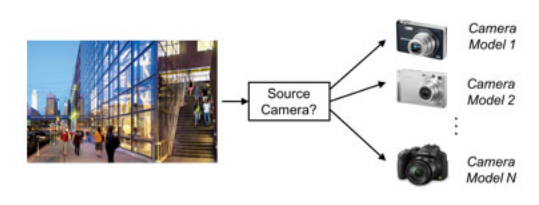
\includegraphics[width=0.99\columnwidth]{pics/model}
	\caption{The problem of identifying a photograph camera source.}.\label{fig:label}  
\end{center} 
\end{figure}   

%%% Add section %%%%%%%%%%%%%%%%%%%%%%%%%%%%%%%%%%%%%%%%%%%%%%%%%%%%%%%%%%%%%%%%%%
\section{Activities}
The best prior solutions to this problem are known to use Deep Neural Networks, as this is a good candidate problem for the number of features it presents on each dataset. Other supervised-learning approaches include Logistic Regression, which was used for this assignment.

As said before, this is a problem which can be cursed with a huge number of features if not approached properly - so it's common in the literature to extract only the noise-features from the images, as it is the real information that can be used to analyse from which camera that picture came from (digital cameras from different models have different fabrication process, which make the noise form each work in different set of conditions).

%%% Add section %%%%%%%%%%%%%%%%%%%%%%%%%%%%%%%%%%%%%%%%%%%%%%%%%%%%%%%%%%%%%%%%%%
\section{Proposed Solutions}
The solution proposed on this assignment is to first extract the right features from the image using noise-analysis, than using Logistic Regression on the data extracted to train and predict correctly the pictures-camera model pairs.

%%% Add section %%%%%%%%%%%%%%%%%%%%%%%%%%%%%%%%%%%%%%%%%%%%%%%%%%%%%%%%%%%%%%%%%%
\section{Feature Extraction}
As said before, the features that have the most physical characteristics information from the cameras are the noise from the picture, so first it should be collected from the dataset.

To make the process faster, and after analysing the test data, the first transformation used on each image was to crop it on the center on a 256x256 subimage. The loss of information in this case won't be as high because most pictures are taken with the focused subject in the center of the picture (or in close proximity), and picture noise is a global characteristic on the picture (influenced by luminosity and reflectivity).

\begin{figure}[!ht]
\begin{center}
	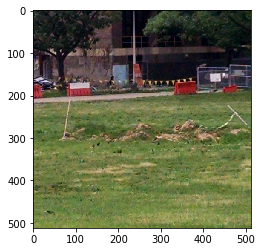
\includegraphics[width=0.99\columnwidth]{pics/original}
	\caption{A cropped image example.}.\label{fig:label}  
\end{center} 
\end{figure}   

Second, a median filter is used on each picture channel to create a new subimage without noise. This new subimage is used to subtract from the original one, creating a picture depicting the noise of the original image.

\begin{figure}[!ht]
\begin{center}
	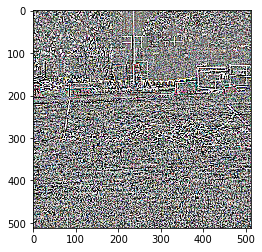
\includegraphics[width=0.99\columnwidth]{pics/noise}
	\caption{The noise image result.}.\label{fig:label}  
\end{center} 
\end{figure}   

It must be noted that figure 3 was prepared for visualization on the report; most of its values were lower than 0 from the subtraction, and only few spots of noise would be visible. This wouldn't influence the Logistic Regression algorithm, as it would normalize the dataset before anyway.

It was used the Median filter in particular because of its properties of filtering salt-and-pepper kind of noise without losing much of contour information, which would make the result 'noised' image more revealing on this aspect.

After getting the noise image, a discrete wavelet transformation was used on it, resulting on a wavelet filtered image and 3 components for each direction gradient. Finally, statistic information is gathered from each channel from the noise and all images resulted from it: the minimum value, the maximum value, mean, variance, skewness and kurtosis. In total, 90 features are extracted from each individual training image ((noise + 4 x wavelet images) x 3 channels x 6 statistic features).

%%% Add section %%%%%%%%%%%%%%%%%%%%%%%%%%%%%%%%%%%%%%%%%%%%%%%%%%%%%%%%%%%%%%%%%%
\section{Logistic Regression}
Using the features extracted, a Logistic Regression model was trained with regularization strength of 1e-5 and maximum number of iterations 100.

\section{Results}
Since the test data didn't have the label for each image, the accuracy was tested using 20\% of the training data after shuffling the order of the images; the coefficients got from the Logistic Regression made 52.35\% of accuracy.

\section{Conclusion}

After setting the use of Logistical Regression as the model for the problem at hand, the most important focus of the analysis was the extraction of features from the training set. Using wavelets, it was possible to replicate information from the images in good amounts, resulting in a fairly successful accuracy for the training data.

Better results could be evaluated by increasing the number of features extracted; other filters besides median could be used, and increasing the number of wavelet filtering on the subimages. As the number of features increased, the PCA algorithm would become necessary as to reduce the dimensionality of the problem.

%%% References %%%%%%%%%%%%%%%%%%%%%%%%%%%%%%%%%%%%%%%%%%%%%%%%%%%%%%%%%%%%%%%%%%%

\end{document}